%----------------------------------------------------------------------------
\chapter{Presentation layer}

The frontend is compiled against Java 21, and is built using multiple libGDX scenes. The program's graphics are completely self-contained, with only a few open-source asset files and fonts required in addition to the declared dependencies -- these are included in the repository.

\section{The rendering pipeline}

The OpenGL pipeline consists of the following steps: vertex processing, vertex post-processing, fragment generation, processing using a fragment shader, per-sample processing\cite{OpenglPipeline}. LibGDX provides calls to the low-level equivalents of each of these steps. As with all other graphics programming problems, the primary objective is to reduce the data sent between the CPU and the GPU, and to minimise GPU context switching.

The GPU may receive information for rendering a model or mesh in two ways. The CPU could pre-calculate everything: model nodes, geometry, normal vectors, materials, colouring, and lighting. For the average programmer, this method is far more desirable. All operations occur in-memory, using a familiar programming language. Crashes are easier to investigate, as the local stack trace can reveal most issues. However, the processor is generally slower at doing matrix calculations. The Peripheral Component Interconnect Express (PCI-e) bus may also become clogged with the transmitted models, and it is already often a bottleneck. If the bus can't deliver frame data from the graphics card to the processor, the image may stall or stutter.

The graphics processor can also be put to work for calculating lighting, shading and orientation. All pipeline steps aside from the first one can be performed using a vertex shader and a fragment shader program. These are written in the OpenGL Shading Language (GLSL)\footnote{\url{https://www.khronos.org/opengl/wiki/Core_Language_(GLSL)}}, which is syntactically based on the C programming language, with subtle changes to allow for a more functional style of data transformation. Incoming vertices are most often moved into place, scaled, and have colours applied to them to create the final look. The PCI-e bus and CPU can focus on other, more specific work, as only the initial vertices need to be sent. Shader optimisation is important in its own right, as it can allow for huge efficiency gains for the entirety of any visual application.

OpenGL is fastest when the type and structure of rendered data does not change. Any settings change or new model may be considered a context change, and can cause frame drops. Batching may be used to combine the geometry of multiple or all models, allowing the GPU to render each frame within the same context. Too many nodes contained in a single model may cause issues though, as a change to any part may require a complete rebuild.

Caching is similar in principle, but more flexible. Instead of rendering the original models, a cache may be created that accounts for layering and invisible faces, dropping anything that isn't needed for a complete image. A cache also requires recompilation when parts of it change.

The processing load may also be reduced by simplifying the scene as much as possible. Objects outside of the current field of view don't need to be rendered, and can be filtered out in a process named culling before the actual render pass happens. The camera's view frustum is the pyramid-shaped area that contains objects actually visible from the current viewpoint. Frustum culling ignores all objects outside this area. Far-away objects can also be rendered at a lower complexity, dropping nodes in order to create lower level of detail (LOD) models. This trades more setup work for better runtime performance.

\section{Low level graphical challenges}

By using near-machine graphical interfaces, we lose some simplified operations, for instance the ability to draw complex three-dimensional shapes directly from code. Most graphics cards have certain predispositions about the data they process, and in low-level cases, our program can't guarantee correct formatting by itself. LibGDX provides access to the GPU's drawing capabilities, but it's the developer's job to use them as expected by the graphics card. This section contains examples for rules that should be followed in OpenGL applications.

\subsection{Triangulation, ear-clipping algorithm}

The triangle are typically used and are a basic, well supported two-dimensional shape on all platforms. Therefore, it's advisable to transform any displayed models to groupings of them.

One geometrically intuitive division operation is the ear-clipping algorithm. An ear is defined as a triangle made up of three successive vertices of a polygon, where the middle vertex is convex -- the internal angle on that vertex must not exceed 180 degrees ($\pi$ radians).\cite{TriangulationByEarClipping} Areas defined by such triples are guaranteed to be subtractable from the polygon's area, since by definition, they can't contain any holes, removing the need to compensate for empty space. The action can then be repeated on the remaining area, each successive step will result in a new triangular piece; when only three vertices remain, we have achieved our goal of subdivision.

The goal of this algorithm is to create a list of vertex indices that should be connected into triangles in order to cover the original polygon fully and efficiently. As a useful side effect, this makes calculating the polygon's area trivial as well.

In the case of libGDX, the EarClippingTriangulator class takes care of this common use case. Following OpenGL idioms, the relevant function requests floating point values (vectors decomposed into their axes), and it results in a list of whole number indices -- every group of three defines a triangle to be created.

\begin{lstlisting}[caption=Example usage of the EarClippingTriangulator class]
    val floats = baseNodes.flatMap { listOf(it.x, it.z) }.toFloatArray()
    val triangles: ShortArray
    val triangulator = EarClippingTriangulator()
    triangles = triangulator.computeTriangles(floats)
\end{lstlisting}

\subsection{Winding order}

Many graphical effects -- including lighting -- require knowledge of the affected faces' normal vectors; a direction that is perpendicular to the whole surface.
When observing the side from this particular direction (meaning that the vector between the camera and a given point of the face can be represented as a multiple of the normal), the apparent size is at its largest -- in layman's terms, we're seeing the front without any rotations around axes that don't match the normal.

The visibility of a polygon can technically also be treated as an effect. To reduce the number of draw calls, it's advisable to only handle faces that have their intended front side visible from the camera's perspective. By default, OpenGL utilises "back-face culling": the spectator can only see shapes where the order of vertices is counter-clockwise (when plotted in relation to the vector connecting the viewpoint and the weighted centre of the polygon). This behaviour can be changed as follows.

\begin{lstlisting}[caption=Example for changing OpenGL's culling properties through libGDX]
    Gdx.gl.glEnable(GL40.GL_CULL_FACE) //enabling
    Gdx.gl.glCullFace(GL40.GL_BACK) //setting filtered side (rear)
    Gdx.gl.glFront(GL40.CW) //changing the intended winding order to clockwise
\end{lstlisting}

\subsection{Using the main thread}

In contrast to the project's simulation module, the user interface is difficult to parallelise. OpenGL functions are usually not thread-safe, requesting and modifying a single graphical context from multiple areas of code is dangerous and will often lead to crashes.

The graphics library abstracts communication with the operating system and GPU as much as possible. In return, it's the developer's responsibility to reduce GPU calls to the absolutely necessary amount. Aside from frame construction, my program mostly uses the main graphical thread for creating unique models and heatmap chunks, as this can't reasonably be done on the CPU.\@I decided against a complex thread-scheduling solution, as the GPU only receives a heavy workload when loading a city from the server, or receiving a heatmap. When programming, I abstracted the render thread for myself using a simple lambda function to obtain the main thread context when needed.

\begin{lstlisting}[caption=Helper function for getting the draw thread]
private suspend fun <T> runOnRenderThread(block: () -> T): T {
        return suspendCoroutine { continuation ->
            Gdx.app.postRunnable {
                continuation.resume(block())
            }
        }
    }
\end{lstlisting}


\section{The main scene}
The program's visual part can be divided into separately rendered modules. The user mostly interacts with the main scene, a view of the currently loaded city. There is no heightmap implementation, buildings are presented at the same height. To understand the details, it is important to know libGDX's hierarchy.\cite{LibgdxModels}

\begin{figure}[!ht]
    \centering
    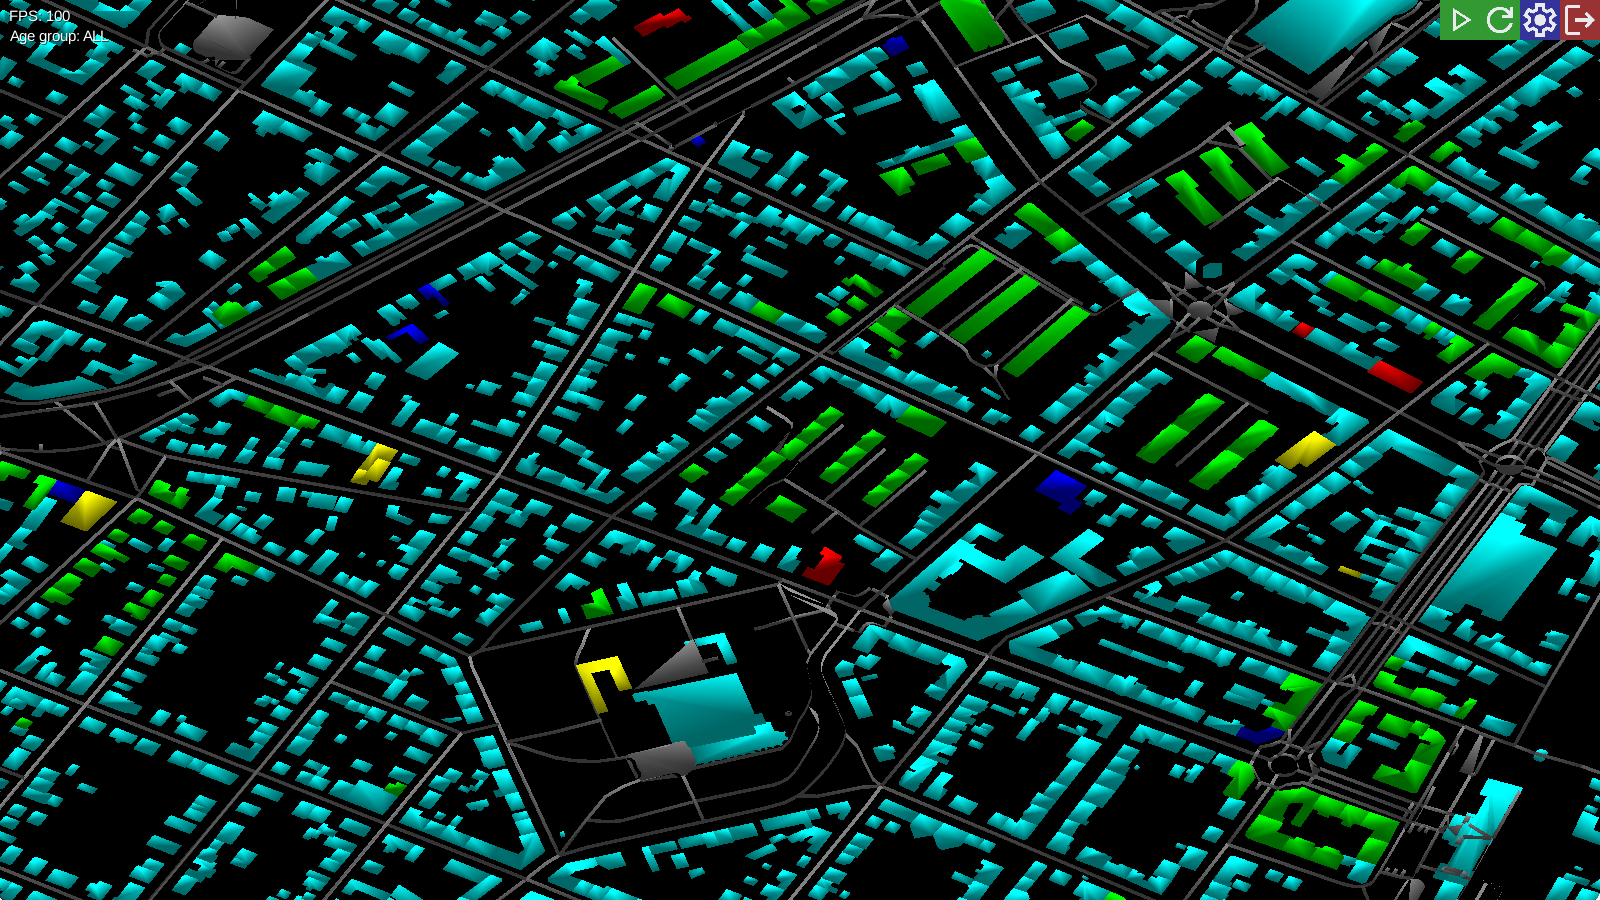
\includegraphics[width=150mm, keepaspectratio]{images/main_graphics_view.png}
    \caption{The main page of the app, with a "false 3D" view}
\end{figure}

The basis of libGDX consists of Nodes, which are a combination of geometry and a material. Nodes may be transformed individually using a 4$\times$4 matrix (Mat4) that determines translation, rotation and scaling. A Node is invisible by itself, but a visual representation can be created by assigning NodeParts (consisting of a MeshPart and a Material) to it. A Material may be an arbitrary texture, but the library also supports simple diffuse, emissive and specular surfaces. MeshParts are collections of vertices in space, with normals attached. These parts can be made using the MeshPartBuilder class, which accepts all OpenGL primitives (such as line strips and triangles). Models are a collection of Nodes, and can be stored in files or created at runtime. A ModelBatch can group multiple drawing operations: every object added to it between its \verb|begin()| and \verb|end()| functions being called is flushed at the end, to be shown at once.

%\begin{figure}[h]
%    \centering
%    \includegraphics[width=100mm, keepaspectratio]{images/map_network.png}
%    \caption{An overview of the network communication required for loading the scene\ \label{simu_network}}
%\end{figure}

I generalised the drawing process by creating a wrapper for instances, the GraphicalObject class. Frustum culling was implemented here using the instance's transformation matrix. Every loaded object is put into one of two child classes for buildings and roads. These wrap the additional OSM API data for later reference.

As a first step, the map needs to be loaded -- as well as the building data, the backend sends over a baseline coordinate pair, calculated as the average of a random sampling of buildings, that can be used as the origin of the graphics scene. This is important as the server should not have any knowledge of the display it's sending data to. Building location data is contained in a batch of BuildingResponse messages and is transformed to be relative to the baseline, then scaled by 100,000. For a building based on a single OSM node, I used a common model, created by the ModelBuilder class's createBox convenience method. For structures represented by a way or relation, the geometry is determined by the outermost way; for these I made three NodeParts, called "top", "bottom", and "sides". The bottom layer is set by unpacking the list of nodes contained in the way. The resulting polygon is sectioned by triangulation and covered by individual triangles, facing the ground. The height is determined by the tags that are also used at the database level. The top layer is a copy of the bottom one, with up-facing normals and the Y-coordinate\footnote{In libGDX, X and Z coordinates use the two axes of the Cartesian coordinate system, with Y representing height} set to the determined height. Side faces are also added using triangles, with each rectangle (formed by two adjacent columns of top and bottom vertices) covered using two of them.

\begin{figure}[!h]
    \centering
    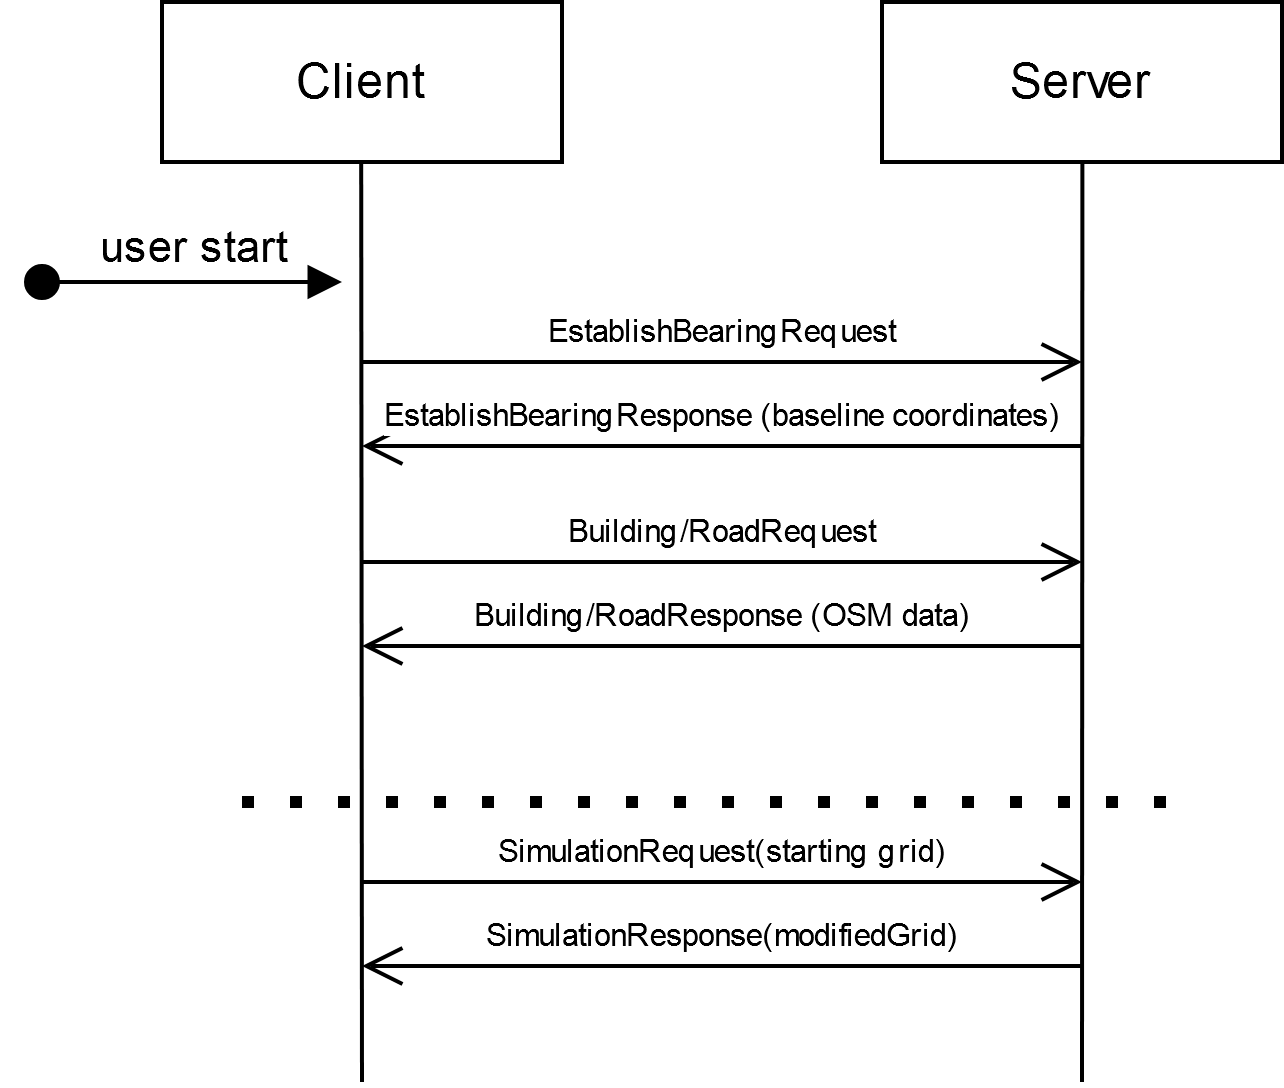
\includegraphics[width=120mm, keepaspectratio]{images/communication.png}
    \caption{Communication between subprojects when loading a map; multiple building and road responses are sent and they may arrive out of order }
\end{figure}

I initially used a simple render loop, opening a ModelBatch and iterating the stored graphics objects; that slowed down after about twenty thousand of them, which is far less than what a typical metropolitan area has. Since frame creation is single-threaded, rendering $n$ objects has a slightly worse than $\mathcal{O}(n)$ time complexity. Instead, I split the playfield into relatively large chunks of 5000$\times$5000 units, which translates to 0.05 degrees of latitude and longitude in my coordinate system. When new data is received, each chunk is transformed into a custom CacheObject -- this wraps a libGDX ModelCache to provide culling and easy identification. Rendering these is much faster, as they're considered static and their contained models are merged and optimised upon creation.\cite{LibgdxModelCache} It makes sense to bake them ahead of time; I initialise the caches when building data is received, as part of the loading process.

Roads are treated as uniform-width lines. Each road is stored as a list of tags and ways which make up the polyline. The points are unwrapped, then two new sets of coordinates are created on the left and right side with a fixed width of 3 units (0.00003 degrees). The resulting strip is then triangulated and added to the scene. All roads have the same light grey colour and are rendered alongside the buildings.

\subsection{Custom camera control}

For libGDX scenes, it is possible to inject a single input processing adapter object, or a combination of multiple objects known as a multiplexer. In the recommended starter 3D program\cite{basic3DlibGDX}, the library's creators added the CameraInputController class; this event handler provides mouse-controlled rotation and zooming for its containing scene.

I created my own camera based on the public InputAdapter interface. The viewing direction is locked for a fixed top-down perspective. The \verb|SmoothMoveHandler| class takes a camera and callback function as input, and can then receive movement commands which are added together. As long as the sum is non-zero, the function is continuously called with a percentage of the current value which is then subtracted. This results in an easing effect, avoiding robotic, sudden direction changes. Since multiple commands may be executed at once, every function that changes the camera's position must be under a mutex (mutually exclusive) lock. Without this, multiple camera location changes cause the currently rendered frame to flicker. The vertical (used keys: W-S), horizontal (A-D) and rotation (Q-E) axes all have dedicated handlers.

Holding the left ALT key and pressing numbers 1--5, the light illuminating the buildings is reduced and the latest heatmap is compiled and displayed over the city. Each button corresponds to one of the simulation's age groups (displayed in the top left corner), with the fifth showing a combination of all maps. Heatmaps have tiles that are coloured by linearly scaling between fully green and fully red, all at half opacity. Tiles with no value are not displayed. The upper threshold is determined by the 95th percentile of all values on the grid to avoid extremely high values in city centres skewing the scale. The resulting float values are passed into a simple vertex shader program. The transformation matrix is set for each cell individually, this is optimised when the program is compiled.

\begin{lstlisting}[caption=Cell colour calculation and the vertex shader program for heatmap cells]
    val strength = (freq.toFloat() / maxFrequency).coerceIn(0f, 1f)
    val red = (strength / 0.5f).coerceAtMost(1f)
    val green = ((1 - strength) / 0.5f).coerceAtMost(1f)
    val color = listOf(red, green, 0f, 0.5f)

    #version 330 core
    in vec3 a_position;
    in vec4 a_color;
    uniform mat4 u_projTrans;
    out vec4 v_color;

    void main() {
        v_color = a_color;
        gl_Position = u_projTrans * vec4(a_position, 1.0);
    }
\end{lstlisting}




\subsection{The menu and popups}

The rest of the rather simple user interface consists of four buttons. The "play" icon is the way to start a simulation, triggering a popup that asks for the required data in five text fields. The start and end times can only ever contain valid ISO format hour and minute values, any other input is ignored. Agent count only accepts numbers. Hitting the \verb|Start simulation| button sends a network message on the currently active websocket, and kicks off the process described in~\ref{simulation-working}. The second, "reload" button is a backup measure to reload the graphics caches if they're in an incomplete state. The third button opens the settings, and the final one gracefully quits the client. The elements are grouped into the GameMenu class and rendered on top the main scene; they each have different colours for inactive, hovered, and pressed states to give feedback. I also made a simple "loading" dropdown that lets the user know they have to wait for some data. All buttons are disabled while loading, except the quit option.

\begin{figure}[!h]
    \centering
    
\includegraphics[width=40mm, keepaspectratio]{images/menu-buttons.png}
    \caption{}
\end{figure}

LibGDX has a mature Scene2D module that helps create two-dimensional overlays and menus on top of existing content. All elements, such as buttons and titles need to be rendered using a skin. Open-sourced examples exist\footnote{https://github.com/czyzby/gdx-skins}, but I decided to create my own in-code. I defined a single basic style for every element. All popups use the resulting Skin, so the entire app's common style can be changed at once in code. The colours are made from a simple tileable 1$\times$1 texture. The icons and fonts are from Google's Material library\footnote{https://fonts.google.com}, packaged with the program.

In the settings popup, the backend's network address can be set, and the \verb|Check| button can initiate a dummy connection to it. If the handshake fails, the button says \verb|Check: Failed|, or \verb|Check: OK| otherwise. A successful check sets the frontend's target to the given address. \verb|Load server| queries the target websocket for map building. \verb|Open file| creates the current system's native file dialog and sends the file selected in it to the database (see~\ref{file-upload}). The menu also describes the basic controls of the program

\begin{figure}[!ht]
    \centering
    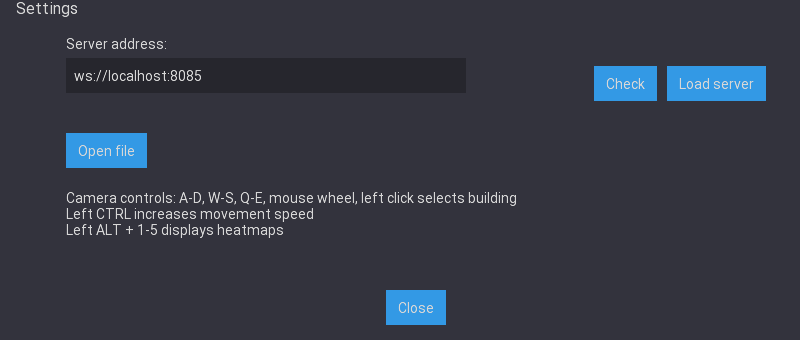
\includegraphics[width=150mm, keepaspectratio]{images/settings.png}
    \caption{The settings page, a popup opened by the "gear" button}
\end{figure}

When clicking on the city view, the camera casts a ray towards the selected pixel. After picking the correct cached chunk from the list, all buildings inside that chunk are collision checked. The first hit causes a popup to appear, with all OSM tags of the building, as well as the calculated capacity listed. This screen is mainly for debugging or trivia purposes as of now. If the ray does not contact anything or another popup is currently open, no window is shown.

\begin{figure}[!ht]
    \centering
    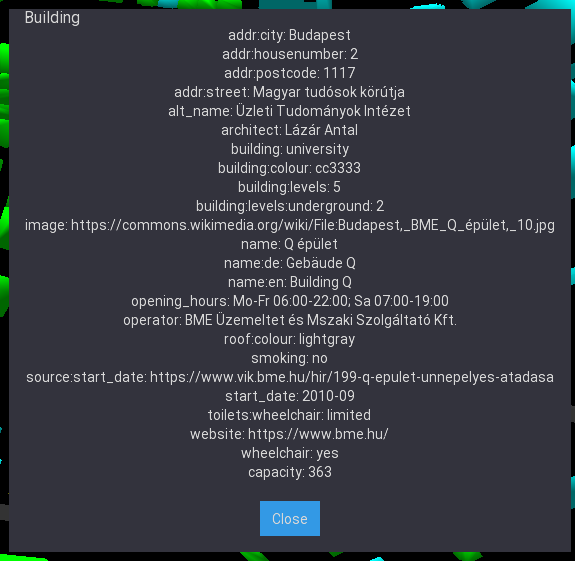
\includegraphics[width=100mm, keepaspectratio]{images/building-popup.png}
    \caption{The building info panel, opened by clicking on a building in the scene}
\end{figure}